\chapter{Projektbeskrivelse}

\section{Projektgennemførelse}\label{Projektgennemfoerlse}
Projektet startede med, at der blev lavet en tidsplan, som var mulig at ændre undervejs, dog med faste deadlines, som skulle overholdes. De forskellige deadlines lagde op til, at der kunne arbejdes efter udviklingsmodeller, som er beskrevet nærmere i metodeafsnittet \ref{Metode}.\\ \\
Tidsplanen blev sidenhen ført mere detaljeret ind i projektstryringsværktøjet Scrum. Scrum blev benyttet til at holde overblikket over manglende opgaver, igangværende opgaver og afsluttede opgaver. Ligeledes blev værktøjet brugt som en kontakt mellem hardware gruppen og software gruppen så begge grupper kunne holde sig opdateret på hinandens opgaver. For at prioriterer arbejdsopgaverne er der blevet benyttet sprints af en uges variehed. Hver arbejdsopgave er blevet prioriteret med et antal point, alt efter hvor tidskrævende opgaven var, hvilket har været bestemmende for hvor mange opgaver, der var mulighed for at lave i hvert sprint.\\
Gruppens seks medlemmer blev fra start delt op i to undergrupper, én med hovedfokus på hardware udvikling, og én med hovedfokus på software udvikling. Dog blev de basic delene til projektet, som kravspecifikation og case udvalgt samlet. Scrum er her også et godt værktøj til at bevare overblikket over de to gruppers individuelle opgaver.\\ \\
Fra start blev der aftalt et ugentlig møde, med vejleder og de to grupper som medvirkende parter. På denne måde blev alle parter holdt opdateres på udviklingsprocessen, især grupperne imellem, men også vejleder. Sidst i forløbet, under test af diverse dele af systemet, blev grupperne samlet og testene blev udarbejdet i fællesskab.\\ \\
Projektet er gennemført ved udarbejdelse af en samarbejdsaftale, herunder udvælgelse af en projektleder, som i tilfælde af uoverensstemmelse havde den afgørende stemme. 

\section{Metode} \label{Metode}
I metode afsnittet beskrives hvilke metoder og modeller, der er blevet brugt til gennemførsel og udvikling af projektet.  
\subsection{Ase-modellen}
Den primære udviklingsmodel, der er benyttet i dette projekt, er ASE modellen. ASE modellen er en udviklingsmodel, der tager udgangspunkt i use cases. 
\begin{figure}[H]
	\centering
	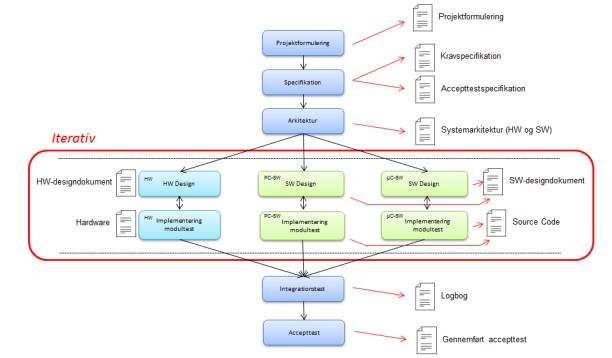
\includegraphics[width=1\textwidth]{Figurer/Metode/ASEmodellen}
	\caption{Projektmodel illustreret med de faser som projektet gennemløber\protect\footnotemark}
	\label{ASEmodel}
\end{figure}
\footnotetext{Fra \textit{"Vejledning til udviklingsprocessen for projekt 2"}}


Modellen er opbygget sådan, at udviklerne benytter vandfaldsmodellen (se afsnit \ref{Vandfald}) til at fastlægge en opgaveformulering, kravspecifikation og systemarkitektur, for derefter at designe og implementere de enkelte moduler i iterationer. \\ Ud fra projektformuleringen specificeres kravspecifikationen som en række use cases. Use cases er et værktøj, der beskriver diverse aktørers interaktion med systemet. Ved at definere kravspecifikationen ud fra use cases, opnås et overblik over hvilke krav, der stilles til systemets endelige funktionalitet.\\ \\ Ud fra kravspecifikationen kan systemets accepttest udarbejdes. Efter kravspecifikationen er fastlagt, udarbejdes systemarkitekturen.\\ I systemarkitekturen uddeles systemets funktionalitet i moduler og deres grænseflader til resten af systemet bestemmes. Ud fra systemarkitekturen designes systemet ved at nedbryde det efter funktionalitet, som kan bindes til både hardware og software.
\subsection{Vandfald}\label{Vandfald}
Denne metode bygger pa at gøre en hel fase af arbejdet færdigt før den næste startes. Grafisk ser det ud som på figur \ref{Vandfaldsmodel}: \\

\begin{figure}[H]
	\centering
	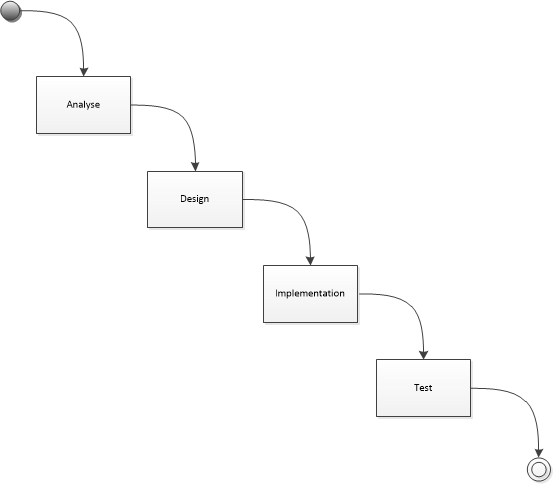
\includegraphics[width=0.8\textwidth]{Figurer/Metode/Vandfald}
	\caption{Vandfaldsmodel}
	\label{Vandfaldsmodel}
\end{figure}
Projektet starter med en analyse, og så videre med de andre faser - design, implementering og test. Det er altså hele systemet, der arbejdes igennem i hver fase, og vandfaldet symboliserer, at der kun arbejdes i en retning, altså man kan ikke gå imod strømmen. Metoden benyttes, når opgaven er veldefineret og velkendt. \\
Projekt forløbet skal have en kort varighed, dvs. mindre end ca. 4 måneder, under velkendte forhold med hensyn til udviklings- og testmiljø, udviklingsmetodik, platforme etc. \cite{Projektledelse}

\subsection{V-model}
V-modellen er en model, hvor testen planlægges parallelt med udviklingen. Accepttesten planlægges detaljeret efter kravnalysen, altså kravspecifikationen, systemtest planlægges detaljeret efter system design, og integrationstesten planlægges detaljeret efter arkitektur design fasen. Unit/modul testen ligger dog uændret i forhold til den traditionelle strategi.
\begin{figure}[H]
	\centering
	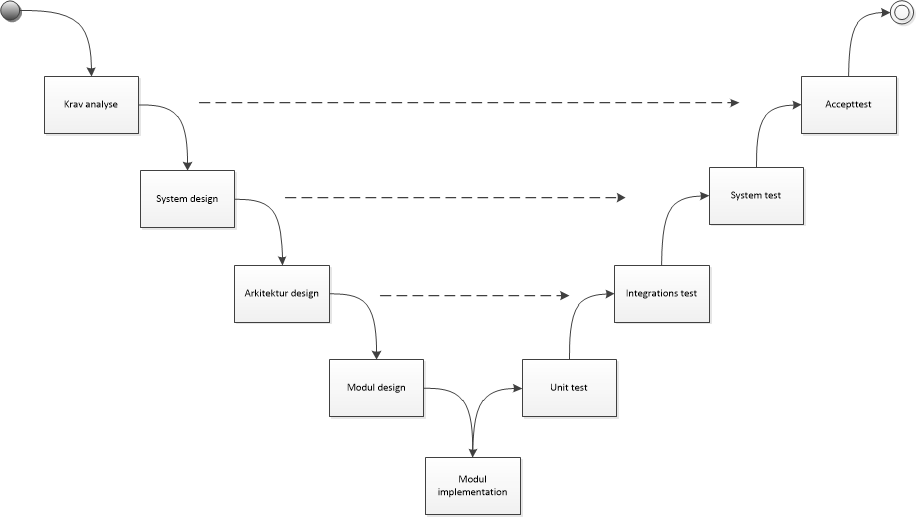
\includegraphics[width=1\textwidth]{Figurer/Metode/Vmodel}
	\caption{V-model}
	\label{Vmodel}
\end{figure}
Testens praktiske udførelse er altså uændret i forhold til Ase-modellen og Vandfaldsmodellen, dvs. den ligger sidst i forløbet. Det betyder at testfaserne planlægges modsat den rækkefølge, de udføres i. Den største forskel for testerne er, at planlægningen baseres på de tidlige modeller af systemet, ikke på det færdige system. \\
 V-modellen udvides desuden med reviews og deadlines (se afsnit \ref{Projektgennemfoerlse}).

\subsection{SysML}
 I beskrivelsen af systemarkitekturen og det detaljerede design for det færdige produkt, er der anvendt SysML. SysML stammer oprindeligt fra UML, dog er UML hovedsagligt centreret omkring udvikling af software systemer. Da det udviklede system både består af hardware og software, er der valgt SysML til beskrivelsen af arkitekturen.\\
Valget af SysML grunder også i, at det giver en god formidling af systemet - dette giver udviklerne et større overblik. Samtidig er det også let for en udenforstående at sætte sig ind i systemets kunnen.\\
I dette projekt er der benyttet struktur- og adfærdsdiagrammer til at specificere og dokumentere systemet. Som strukturdiagram er der anvendt et blok definitions diagram (bdd) samt interne blok definitions diagram (ibd).\\
Der er anvendt adfærdsdiagrammer i form af sekvensdiagrammer i dette projekt. Disse diagrammer er velegnet til sekventielt at beskrive den logiske funktionalitet i systemet. Softwaren er opbygget ud fra sekvensdiagrammer beskrevet i design afsnittet.

\section{Specifikation og analyse}
Overvejelserne omkring designet af softwaren inden opstart på implementeringen var, at systemet skulle opfylde de opstillede krav i kravspecifikationen samt have en god brugergrænseflade.\\
Det blev hurtigt klart, at hvis software systemet skulle fungerer som ønsket ville det blive nødvendigt at implementerer systemet vha. tråde. Dette var nødvendigt da der løbende var flere funktioner, der kørte samtidig. På den måde ville det være en god måde at forøge udnyttelsesgraden af systemet.\\
Tankerne om designet af brugergrænsefalden var at tage udgangspunkt i de 16 principper for gode brugergrænseflader. Ud fra disse principper blev designet af brugergrænsefladen udfærdiget til at være eneklt og brugervenligt for brugeren. Herud over gik designet på at få brugergrænsefladen til at se så virkelighedsnær ud som muligt. Derfor blev der lavet reasearch omkring blodtryks monitorer hvorefter systemets brugergrænseflade er designet ud fra disse oplysninger. 
 
I udviklingen af hardwaren, var der behov for, at mange af komponenterne blev nødt til at blive taget op til genovervejelse. \\
Der blev valgt at bruge en instrumenteringsforstærker til forstærker-blokken, i stedet for en operationsforstærker, grundet instrumenteringsforstærkerens reelle komponents tætte relation, til dens ideelle modpart. Da der blev arbejdet med meget små spændinger, så var det vigtigt med en stor indgangsimpedans, for at kunne forstærke disse små spændinger. Andre fordele ved instrumenteringsforstærkeren indebærer let justerbar gain, samt høj common mode rejection ratio. \\
Dynamik området ved forstærkeren, blev oprindeligt fastlagt til at være højere, end det endelige fastlagte dynamikområde. Dette blev justeret, fordi strømforsyningen og det oprindelige dynamikområde, lå for tæt på hinanden. Det endelige dynamikområde blev valgt ud fra dynamikområderne til rådighed, i vores DAQ. \\
Filterets overordnede design og komponenter, var givet fra de krav, der var blevet sat til hardwaren fra starten af, og der var derfor ikke meget plads til ændringer af designet. Som spændingskilde blev Analog Discovery valgt, i stedet for et batteri, da Analog Discovery giver en stabil strøm, som ikke har behov for at blive afbalanceret. \\

\chapter{Design, implementering og test}
   
\section{Hardware design}
I dette afsnit beskrives udarbejdelsen af hardware design, og tilhørende tanker.

Der blev bestemt tideligt i forløbet at dele hardwaren op i to dele, en forstærker del og en filter del. 
\\
\begin{figure}[H]
	\centering
	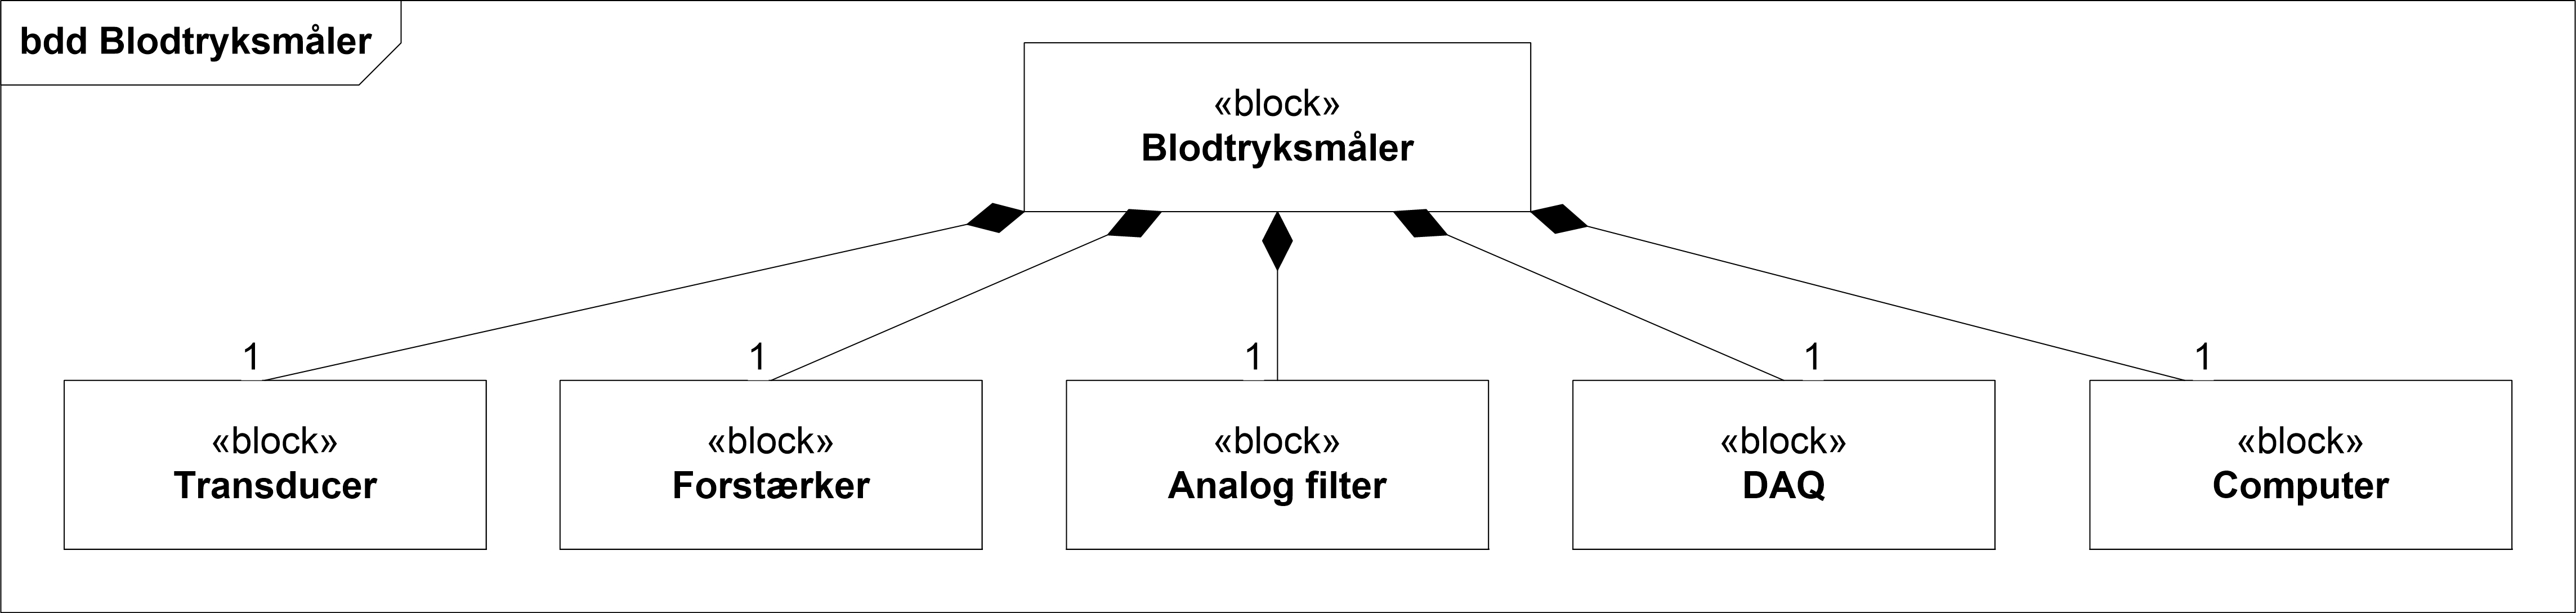
\includegraphics[width=1\textwidth]{Figurer/Hardware/BDD1}
	\caption{Blokdiagram for blodtryksmåler systemet.}
	\label{rBDD blodtryksmaaler}
\end{figure}

Ud af blokdiagrammet, figur \ref{BDD blodtryksmaaler}, kan man se at blodtryksmåler systemet består af fem dele. En transducer, som omformer tryk til spænding, en forstærker, et analogt støjfilter, en DAQ og en computer. \\

Det første der blev designet til fulde, var forstærkeren. Forstærkeren blev designet, med tanke på, at det er meget små spændinger, som ville blive målt fra transduceren. En almindelig operationsforstærker blev derfor fravalgt, og en instrumenteringsforstærker blev valgt i stedet. Vejleder anbefalede at typen INA114 af vejleder, grundets denne type's gode common mode rejection faktor, og høje reelle indgangsimpedans. Kredsløbet blev som vist på figur \ref{forstkreds}. \\

\begin{figure}[H]
	\centering
	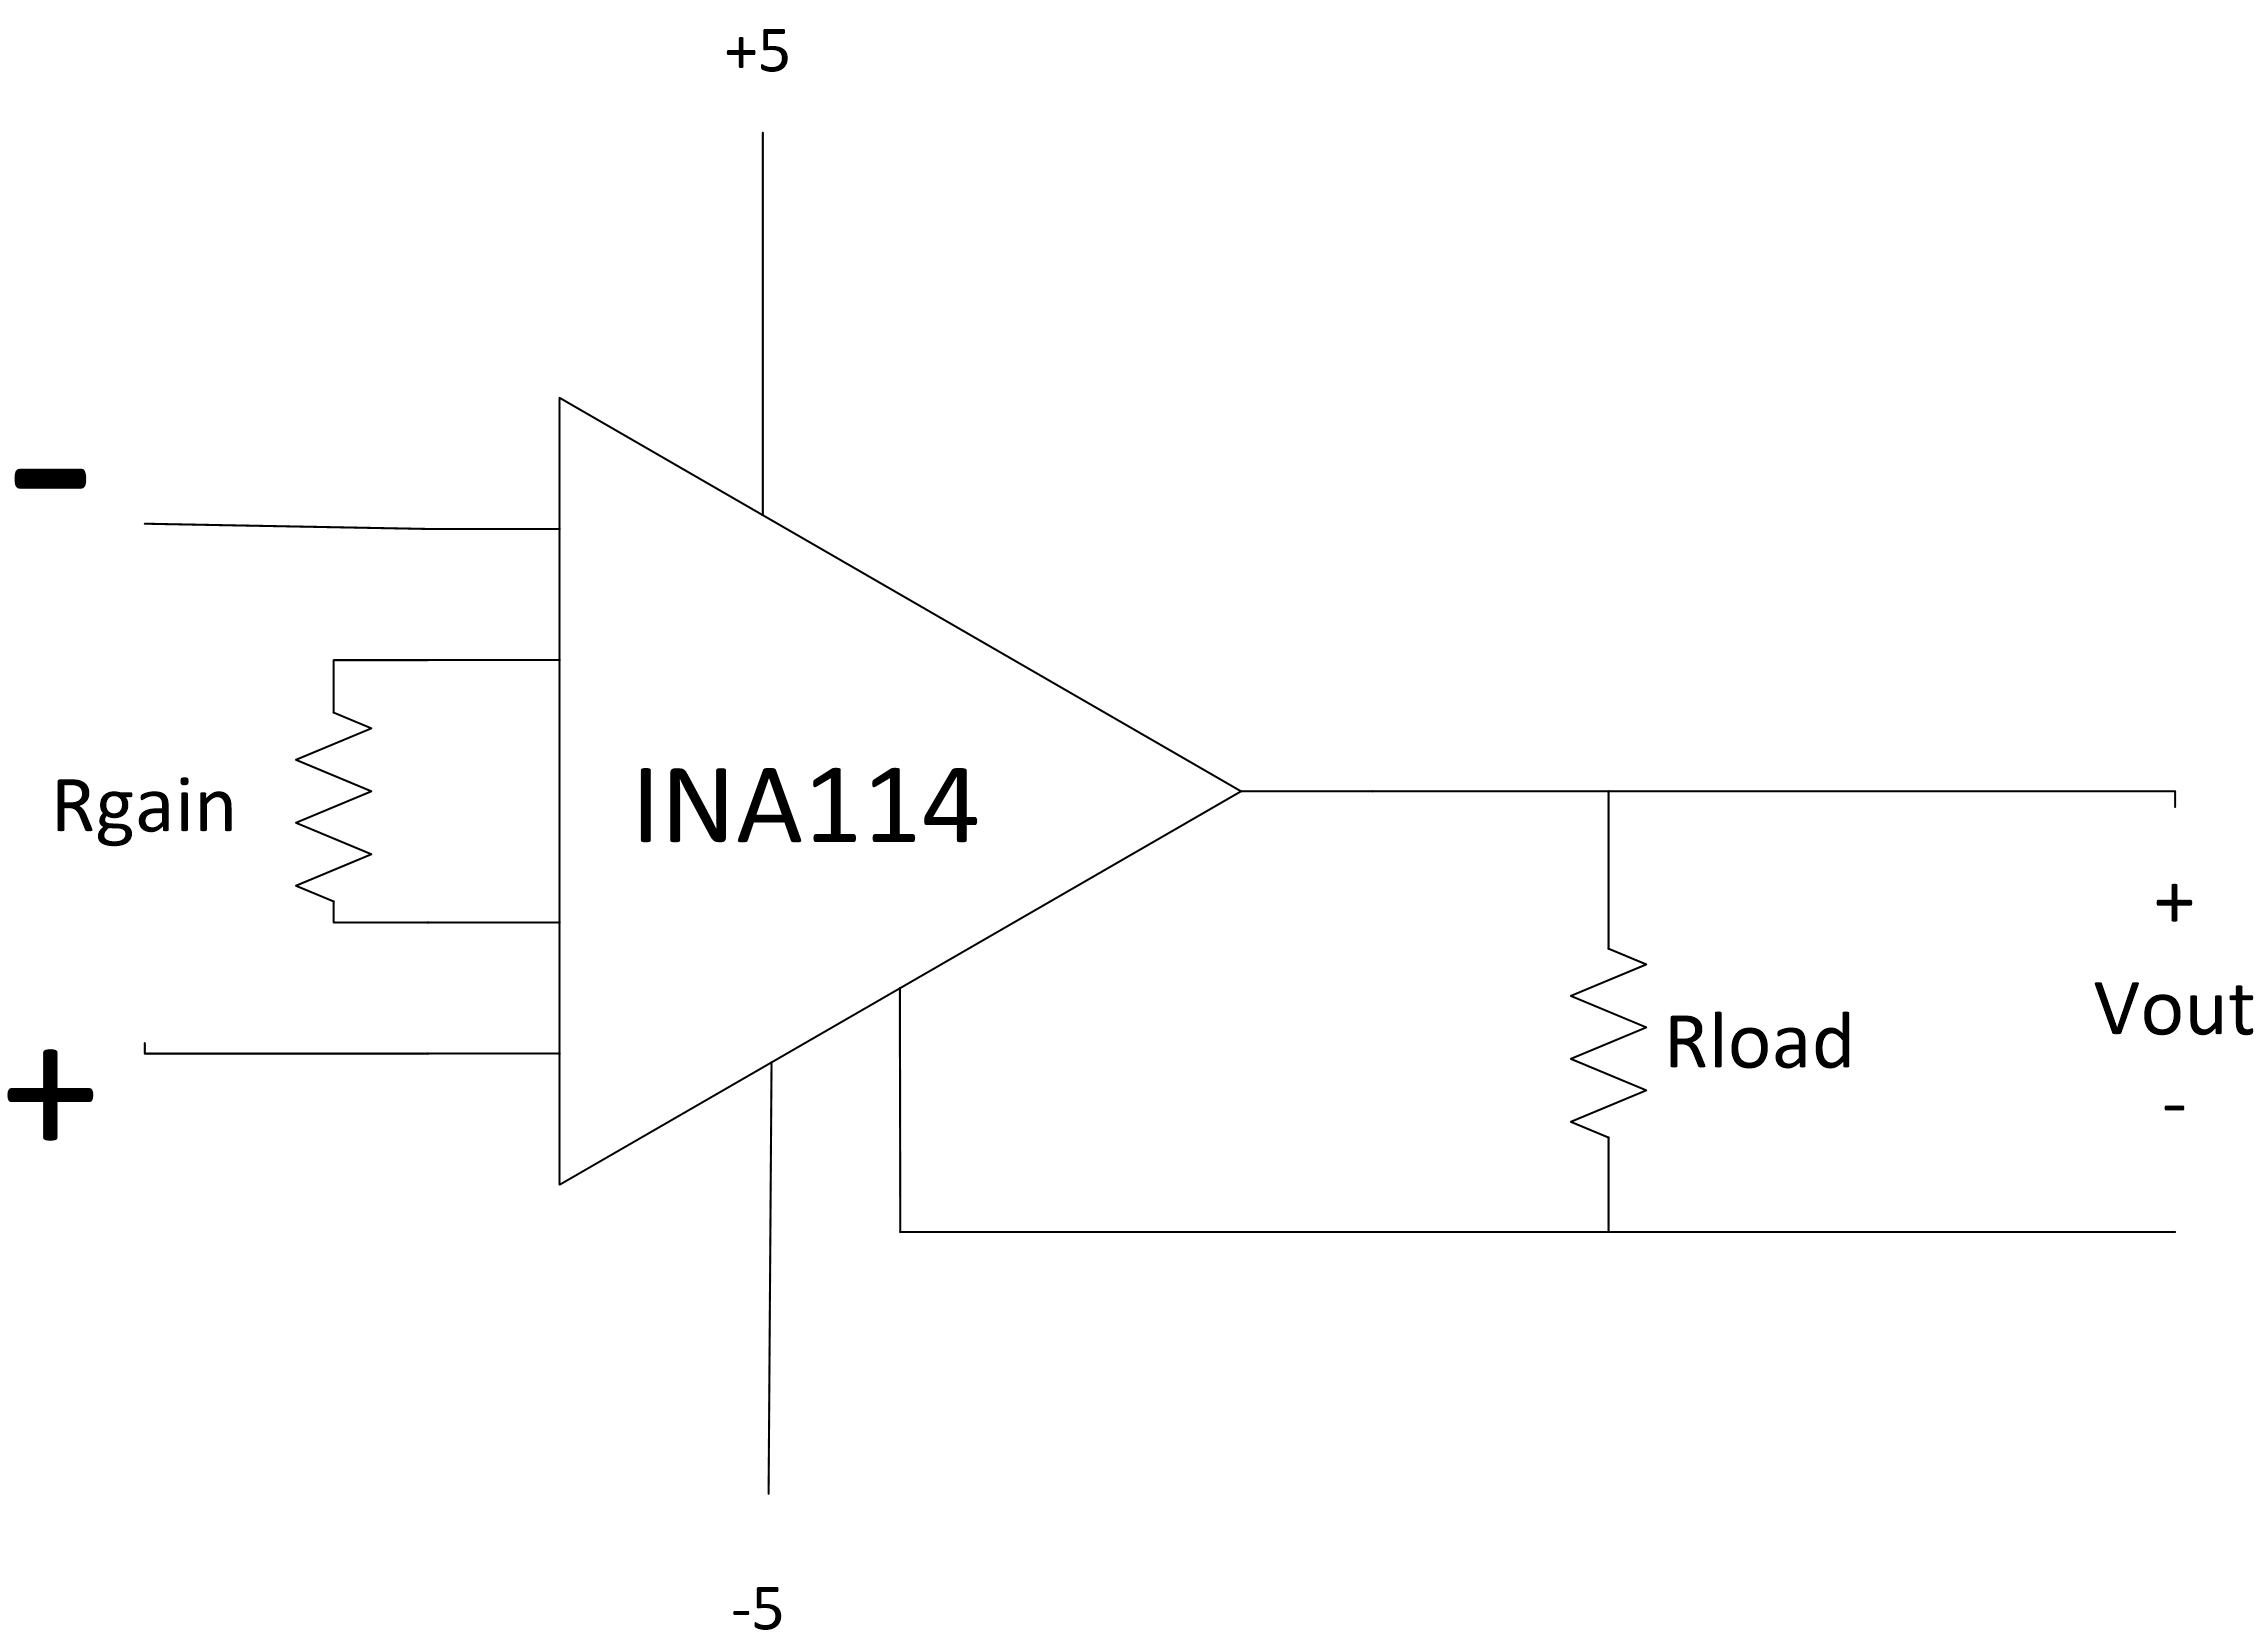
\includegraphics[width=0.6\textwidth]{Figurer/Hardware/Forstaerker}
	\caption{Der overordnede design af forstærkeren.}
	\label{forstkreds}
\end{figure}

Som set på figur \ref{forstkreds}, så er R$_{gain}$ modstanden som bestemmer forstærkningen, og R$_{load}$ repræsentere den belastning der kommer efter forstærkeren. 

Komponentværdier for forstærker er herefter udregnet. Disse udregninger kan ses i dokumentationen, afsnit xx, og komponentlisten for forstærkeren kan ses i afsnit \ref{himpl}, længere nede. 

Det næste der skulle designes, var filteret. Filteret skulle realiseres som et aktivt 2. ordens lavpasfilter af typen Sallen-Key med unity gain, og med en båndbredde på 50 Hz. Kredsløbet kan ses på figur \ref{fig:Filter}. Filteret blev yderligere specificeret til at skulle være et Butterworth filter, med en cutoff frekves på 50 Hz. Yderligere var visse komponentværdier forhåndsbestemt. Designet af filteret kan ses på figur \ref{fig:rFilter}.

\begin{figure}[H]
	\centering
	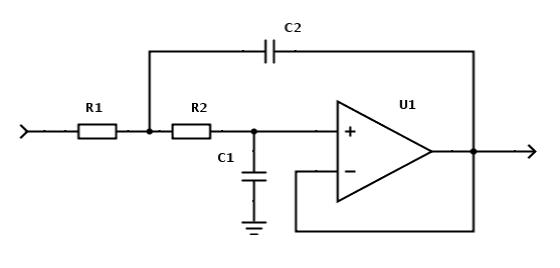
\includegraphics[width=1\textwidth]{Figurer/Hardware/FilterDesign}
	\caption{Unity gain 2. ordens Sallen-Key lavpas konfiguration}
	\label{fig:rFilter}
\end{figure}

Et Sallen-Keyfilter har en anderledes $\zeta$ , grundet anderledes prioriteter, i forhold til frekvensområdet. Der blev brugt en hjemmeside til at finde overføringsfunktionen for det givne filter \cite{overforing}. Herefter blev komponentværdierne teoretisk udregnet. Udregningerne kan ses i dokumentationen, afsnit xx. De endelige værdier for komponenterne, kan ses på komponentlisten for filteret i afsnit \ref{himpl}. 
   
   
\section{Software design}\label{Software arkitektur}
   I software designet er der udarbejdet en domæne model, der giver et overblik over hele systemet.
   
 \begin{figure}[H]
	\centering
	\includegraphics[width=1\textwidth]{Figurer/ISE/Domaenemodel}
	\caption{Domænemodel}
	\label{domaenemodel}
\end{figure}

I domæne-modellen er relationerne mellem aktørerne og systemets dele beskrevet med pile og vejledende tekster - dette skulle gerne give et større overblik over systemets funktionalitet. \\ 
En domænemodel beskriver dog ikke, hvilken rækkefølge de forskellige handlinger sker i, og derfor er der udarbejdet sekvensdiagrammer for hver use case for systemet, som skal beskrive dette.\\
Nedenfor på figur \ref{sekvensdiagram} ses sekvensdiaframmet for use casen "Mål blodtryk":

\begin{figure}[H]
	\centering
	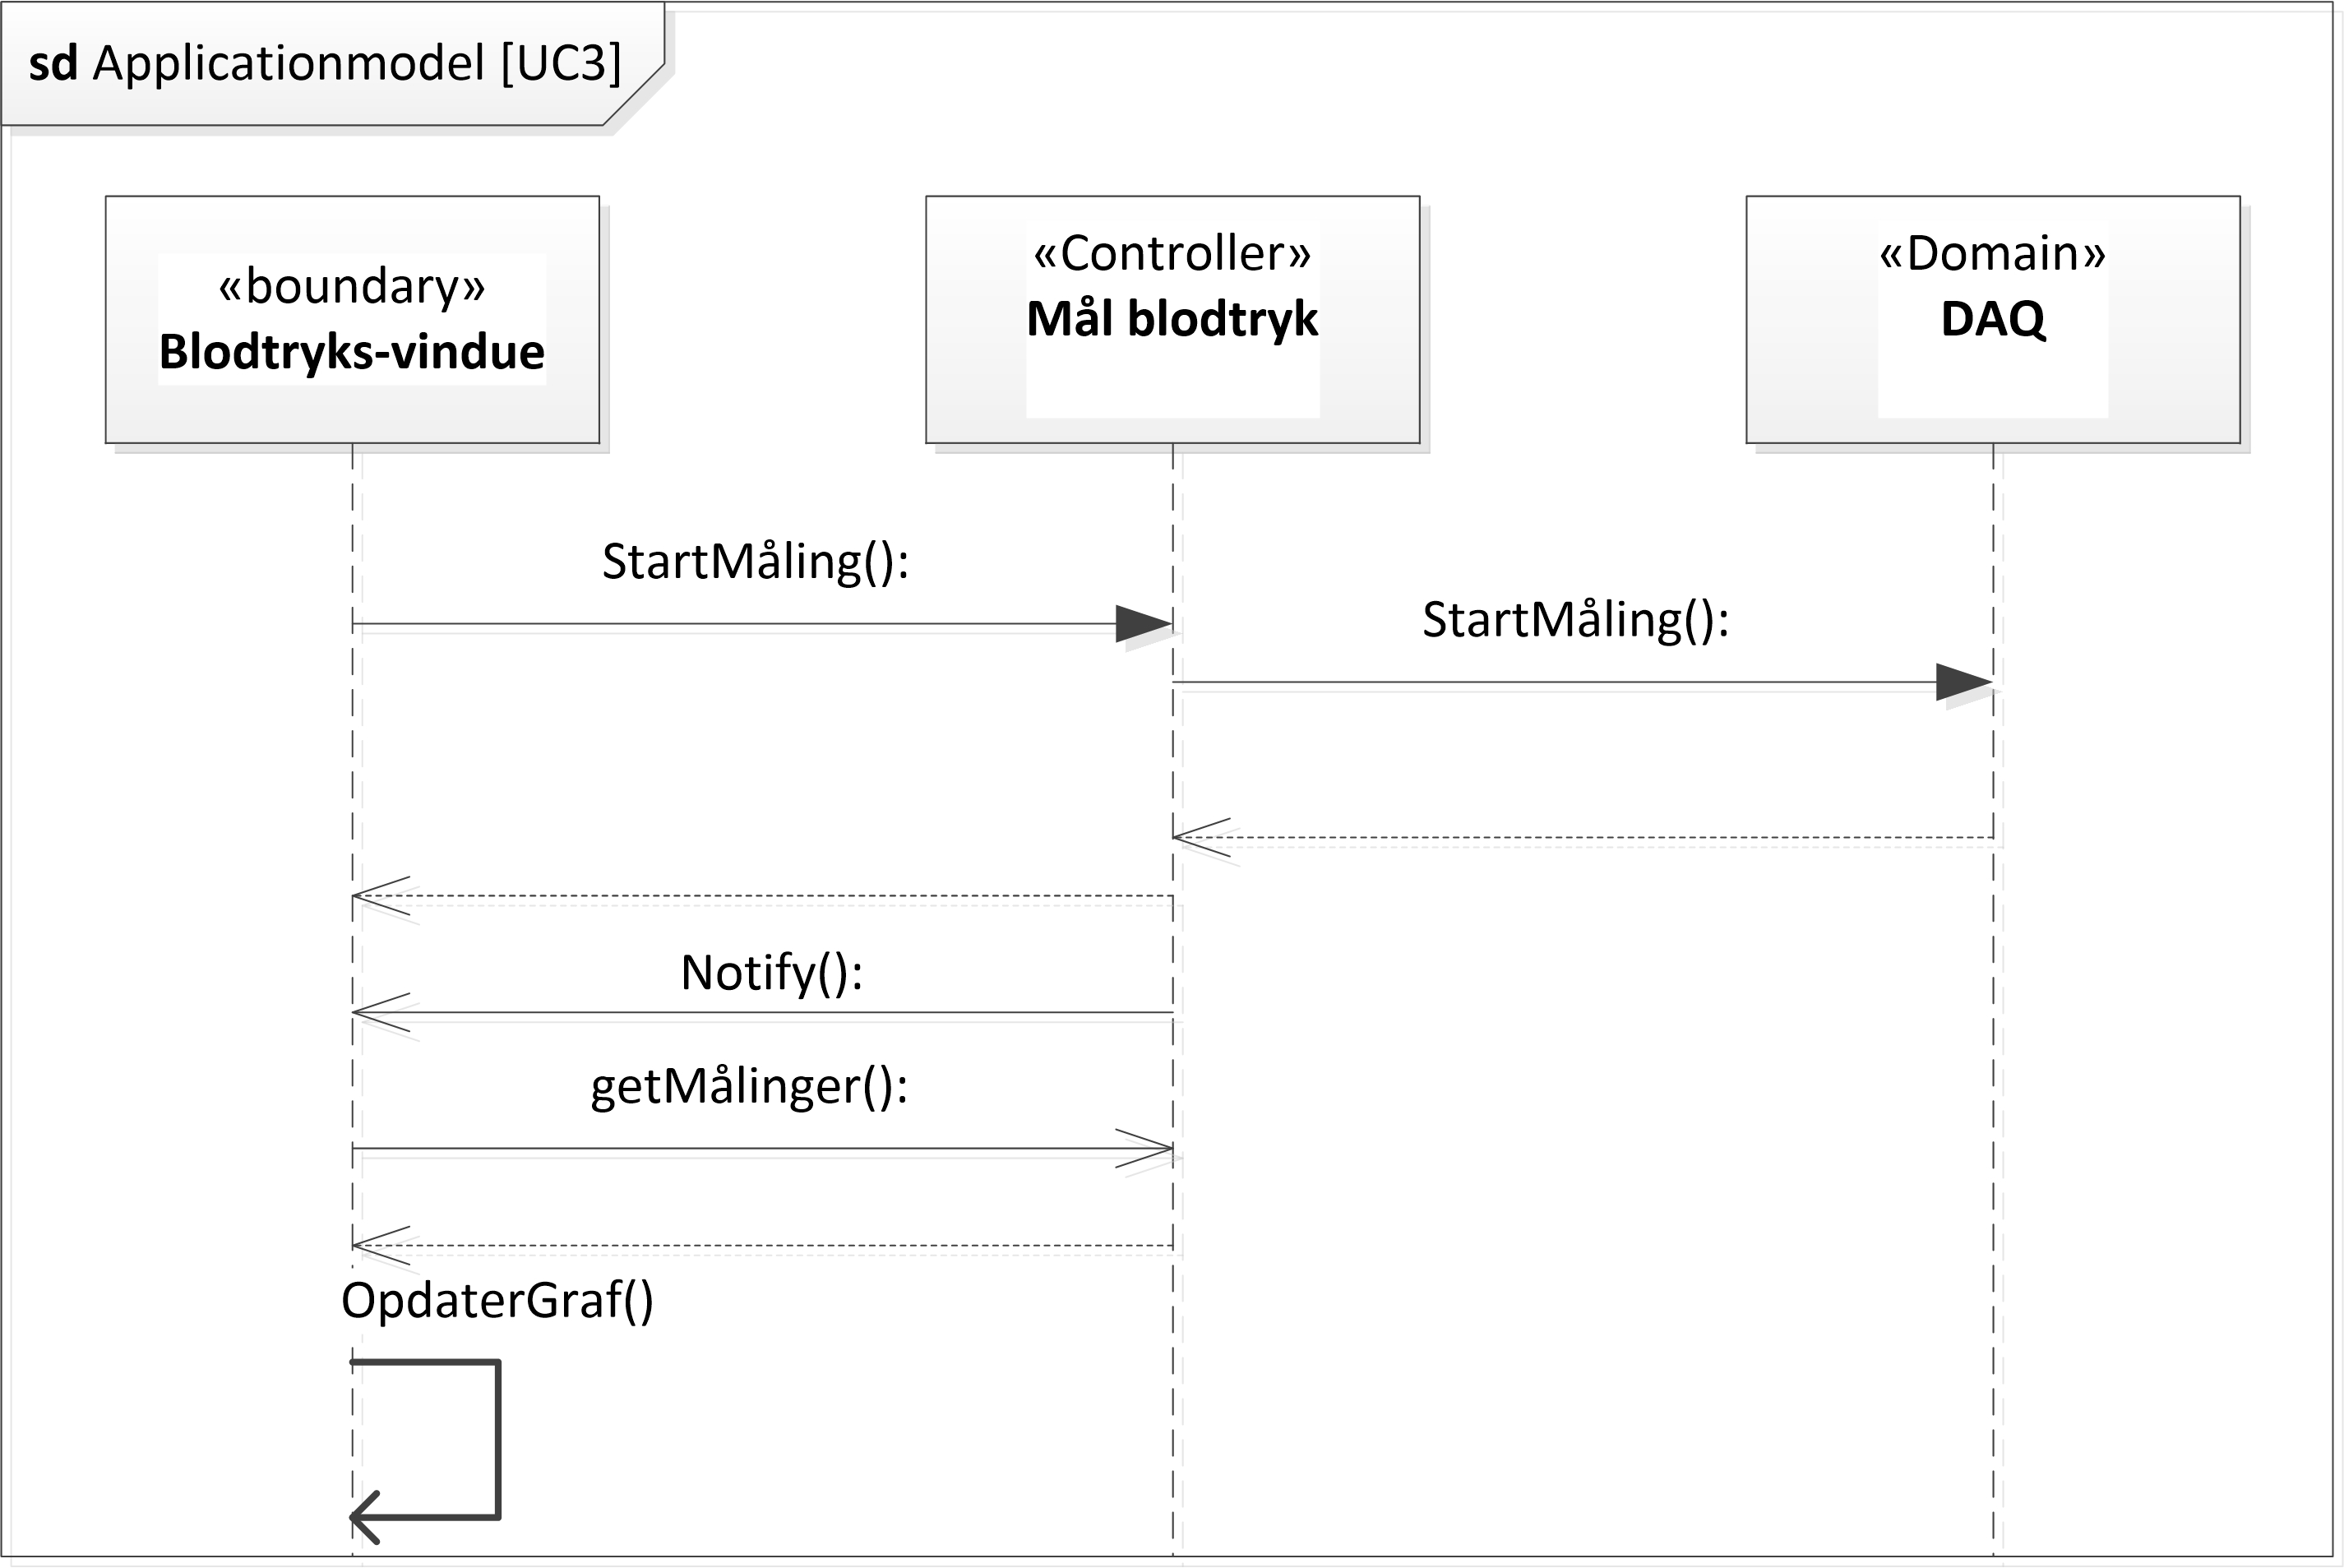
\includegraphics[width=1\textwidth]{Figurer/ISE/sdAppModelUC3}
	\caption{Sekvensdiagram UC3}
	\label{sekvensdiagram}
\end{figure}

Figur \ref{sekvensdiagram} viser hvordan brugeren interagerer med brugergrænsefladen ved at starte blodtryksmålingen. Herefter bliver metoden til at starte blodtryksmålingen kaldt ned gennem logik- og datalag hvor efter målingen vises i en graf på brugergrænsefladen. Grafen bliver hele tiden opdateret med nye målinger.\\
Ud fra dette kan det ses hvordan brugerens interaktion med brugergrænsefladen sætter gang i metoder i software programmet. Skevensdiagrammet giver altså et overblik over hvordan softwaren er bygget op.\\
Sekvensdiagrammerne for de øvrige use cases kan ses i dokumentationen afsnit \textbf{Afsnit i dokumentation}
  

\section{Hardware implementering}
\label{himpl}
Efter komponentudregningen, byggede gruppen de to hardware blokke op. Der blev valgt at bygge forstærkeren og filteret seperat, grundet pladsmangel og sammenhæng.\\

\begin{figure}[H]
	\centering
	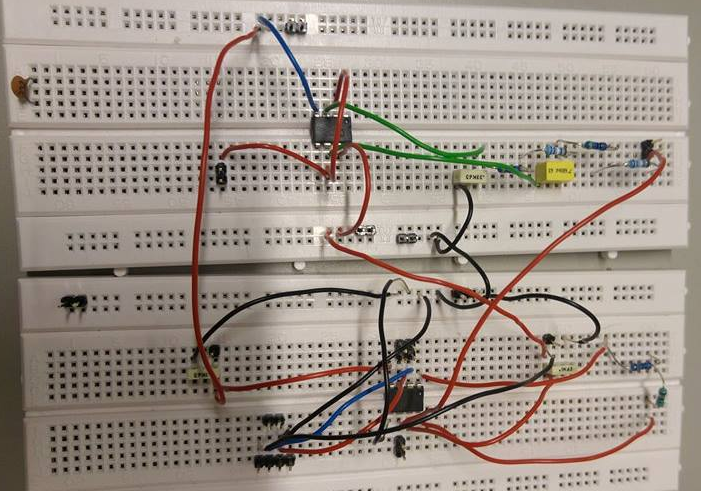
\includegraphics[width=1\textwidth]{Figurer/Hardware/samletopstilling}
	\caption{Opstilling af forstærker og filter}
	\label{samletopbygning}
\end{figure}

Grundet mangel på præcise modstande, bedømte gruppen at det var bedst at bygge modstandende i forholdsvist filteret og forstærkeren, op i to, så det var muligt at komme så tæt på den ønskede modstandsværdi som muligt. \\
For forstærkeren, blev styklisten som vist på tabel \ref{forsttabel}.



\begin{table}[H]
\centering
\begin{tabular}{lllll}
\textbf{Komponent} & \textbf{Antal} & \textbf{Type}  &  &  \\ \cline{1-3}
Modstand           & 1              & 120 $\Omega$   &  &  \\ \cline{1-3}
Modstand           & 1              & 4.8 $\Omega$   &  &  \\ \cline{1-3}
Kondensator        & 2              & 100 nF         &  &  \\ \cline{1-3}
Instrumentationsforstærker &    1   & INA114		     &  &  \\ \cline{1-3}
\end{tabular}
\caption{Forstærkertabel}
\label{Forsttabel}
\end{table}

Grundet forskel imellem teoretiske værdier og fysiske, er R$_{gain}$ 0,51$\Omega$ mindre end den skulle have været.\\

Den samlede stykliste for filteret blev som vist på tabel \ref{Filtertabel}.

\begin{table}[H]
\centering
\begin{tabular}{lllll}
\textbf{Komponent} & \textbf{Antal} & \textbf{Type}  &  &  \\ \cline{1-3}
Modstand           & 2              & 6.2 k $\Omega$ &  &  \\ \cline{1-3}
Modstand           & 2              & 470 $\Omega$   &  &  \\ \cline{1-3}
Kondensator        & 1              & 680 nF         &  &  \\ \cline{1-3}
Kondensator        & 1              & 330 nF         &  &  \\ \cline{1-3}
Operationsforstærker &    1         & OP27G          &  &  \\ \cline{1-3}
\end{tabular}
\caption{Filtertabel}
\label{Filtertabel}
\end{table}

I det analoge filter, er kondensatoren, C$_1$, i praksis 3,2 nF mindre end  beregnet. Desuden er de to identiske modstande, R$_1$ og R$_2$, som i praksis er 17$\Omega$ mindre end teorien foreskriver.\\
Der blev vurderet at afvigelserne var forholdsvidst små, og derfor er der valgt at se bort fra dem. For modstandende er der desuden 1 procents usikkerhed, hvilket betyder man alligevel ikke kan være helt sikker på komponentværdien.\\
En reel cutoff frekvens blev herefter udregnet af gruppen. Denne kan ses udregnet på figur \ref{cutoff}.


\begin{align}
f_{c} = \frac{1}{2\pi \sqrt{R_{1}C_{1}R_{2}C_{2}}} = \frac{1}{2\pi \sqrt{6687 \cdot 333,2\times 10^{-9} \cdot 6687 \cdot 680\times 10^{-9}}} = 50,37 Hz
	\label{cutoff}
\end{align}
%\caption{Udregning af den reelle cutoff frekvens}

\section{Software implementering}
I software implementeringen er der blevet beskrevet hvordan systemet er blevet implementeret i form af teoretiske metoder og kode udsnit samt diagrammer over den implementerede kode.
\subsection{3 lags modellen}
Softwaren er implementeret først og fremmest ud fra 3-lagsmodellen 3-lagsmodellen er
bestående af lagene præsentationslag, logiklag og datalag. Denne opdeling af lagene gør
det langt lettere at vedligeholde systemet fordi der kan ændres i et enkelt lag uden det har
indflydelse på resten af programmet.
Det er desuden en god software arkitektur at bruge ved et system udarbejdet af en gruppe,
da der kan arbejdes på to forskellige lag af to personer samtidigt, hvis bare grænsefladerne
bliver overholdt.\\
Herudover har vi implementeret koden så den har lav kobling og høj samhørighed så der har været mulighed for at teste kode elementer undervejs i processen. 

\subsection{Tråde}

\subsection{Observer}

\subsection{Kode elementer}

\subsection{Software diagrammer}

\section{Test}
Der er løbende blevet lavet test på systemet i form af unittest, modultest, integrationstest og slutteligt accepttesten, som blev udført under observation af vejleder.\\ 
I de indledende modultest af hardware blev det eftervist at forstærkeren har en forstærkning på tilnærmelsesvis 400 gange forstærkningen. Ligeledes opfyldte det analoge filter tilnærmelsesvis kravet om, at have en knækfrekvens på 50 Hz, idet modultesten af filteret viste, at den reelle knækfrekvens ligger lidt over 50 Hz. Ved de senere integrationstests af hardwaren blev det eftervist at forstærkeren og det analoge filter virker efter hensigten når disse er koblet sammen. I den sidste integrationstest af hardwaren blev det vist, at systemet med stor nøjagtighed i forhold til teorien kan levere et spændings output svarende til det tryk input som transduceren leverer.\\
SOFTWARE!!!
Ved integrationstesten af systemet kunne det ses, at værdierne der blev opfanget i programmet, passede nogenlunde overens med de værdier som kunne ses vha. oscillopet i Analog Discovery. Dette galdt både værdierne for det atmosfæriske tryk og væsketrykket i søjlen. Desuden kunne det ses at programmet viste et blodtryk i mmHg som tilnærmelsesvist var lig det teoretiske tryk udregnet i væskesøjlen. \\
Ved accepttesten blev samtlige krav fra kravspecifikationen testet. Analog Discovery's signalgenerator blev sluttet til forstærkeren som var forbundet til det analoge filter. Fra det analoge filters udgang var der forbindelse til DAQ'en som havde forbindelse til en computer, hvor programmet var kørende.\\
Fra Analog Discovery blev systemet påtrykt et blodtrykssignal fra en rotte. På baggrund af denne opstilling blev use case 4, 5 og 6 testet og godkendt.\\
Til test af use case 1, 2 og 3 blev Analog Discovery udelukkende brugt som spændingskilde. En vandsøjle med kendt tryk blev koblet til en transducer der blev koblet til systemet. Disse tre use cases blev lige ledes gennemført og godkendt. For dybere beskrivelse af test se test afsnit (afsnit 5) og accepttest afsnit (afsnit 6) i dokumentationen.

\section{Resultater og diskussion}
Hovedkravene til dette projekt var at udarbejde et elektronisk kredsløb med indbygget analogfilter og en forstærker, der forstærker signalet fra en transducer. Yderligere var der krav om at udforme en software, som kunne afbillede signalet fra hardwaren grafisk og som funktion af tiden. Desuden var der yderligere en række krav til softwaren, specificeret i afsnit \ref{Krav}. Det lykkedes at udarbejde et produkt, som opfylder alle disse krav. \\[1ex]

For at sikre systemet mod "ulovlig"\ indtrængning skal man igennem et login system, hvorefter det er muligt at starte en blodtryksmåling. Der kunne til fordel være implementeret en funktion, som gav mulighed for at igangsætte en blodtryksmåling uden om login i tilfælde af en akut sag.\\ 
Selve blodtrykssignalet vises i blodtryksvinduet som funktion af tiden, dog uden akse benævnelser på grafen, som vist på figur \ref{blodtryk}:

\begin{figure}[H]
	\centering
	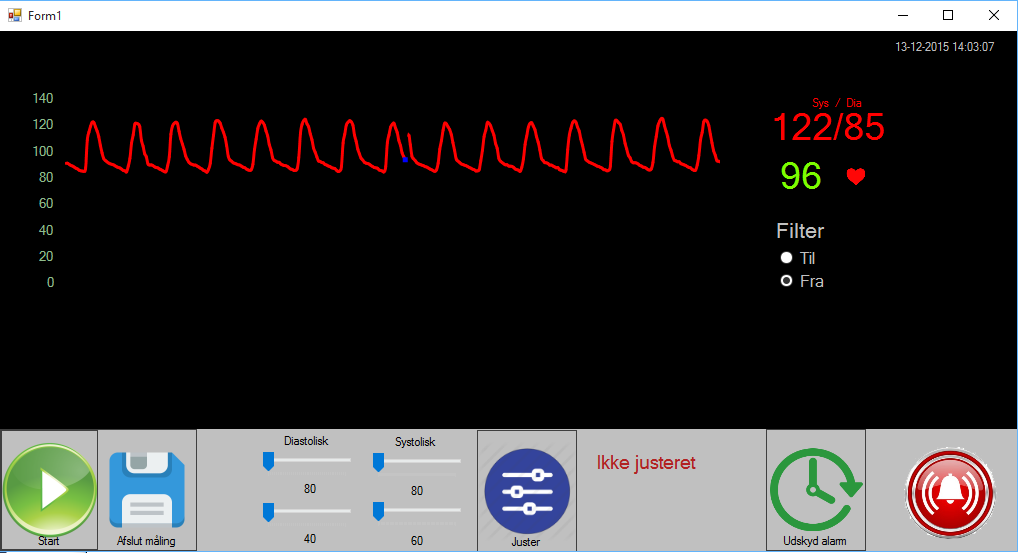
\includegraphics[width=1\textwidth]{Figurer/SoftwareImplementering/blodtryk}
	\caption{Blodtryskmåling}
	\label{blodtryk}
\end{figure}

\textbf{Skriv omkring at tidsaksen er forsinket}
På figur \ref{blodtryk} ses det, at det er lykkedes implementere funktioner, som digitalt filter, alarmering og visning af systole, diastole og puls\\
Efter foretegaet måling er det muligt at gemme data med tilhørende informationer i en lokal database, hvilket er afbilledet på figur \ref{databasegem}:

\begin{figure}[H]
	\centering
	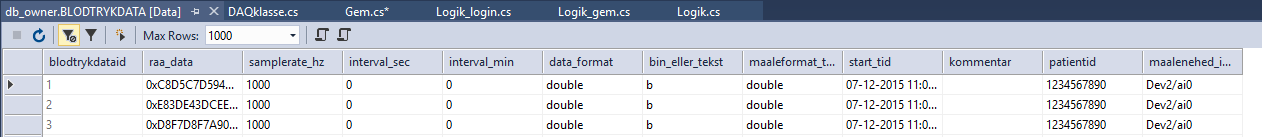
\includegraphics[width=1.1\textwidth]{Figurer/SoftwareImplementering/databasegem}
	\caption{Målinger i databasen}
	\label{databasegem}
\end{figure}

Signalet fra transduceren bliver igennem hardwaren henholdsvis forstærket og filtreret. Igennem forstærkeren har et krav været at den skulle forstærkes 400 gange. Igennem test kan det ses at der tilnærmelsesvis opnås en forstærkning på 400, med forbehold for måleusikkerheder. Et problem har været, at Analog Discovery’s måle scopes på indgangene ikke har kunnet opfange den størelse signaler der arbejdes med grundet Analog Discovery’s offset. Når der tages højde for offset nærmede den målte forstærkning sig 400. \\
Et krav til det analoge filter var at den skal have en knækfrekvens på 50 Hz. Ved modultesten kunne det ses, at knækfrekvensen minimalt oversteg de 50 Hz, hvilket skyldtes at der ikke arbejdes med ideelle komponenter. Dog stemte målte amplitudekarakteristik overens med den teoretiske. \\
Da forsygningsspændingen var +/- 5V kunne forstærkerens udgangssignal ikke være højere end ca. 4,2V og filterets udgangssignal kunne ikke være højere end ca. 3V. Dette medførte at signalet endte med en spædning på +/- 3V. Herefter, for at kunne udnytte DAQ’ens dynamikområde bedst, blev signalet sat maksimalt +/- 2,5V, svarende til en indgang på DAQ’en. Ved valg af en større forsyningsspænding ville signalet være blevet forstærket yderligere, således at signalet kunne sendes ind på én af de højere indgange med +/- 5V. Dette kunne føre til en bedre udnyttelse af DAQ'ens dynamikområde.\\
\\
Gennemgang af alle krav til læses i dokumentationen afsnit ???, samt yderligere forbedringer til systemet kan læses i afsnit \ref{fremtid}.
\section{Opnåede erfaringer}
I løbet af projektet, er der generelt opnåede erfaringer omkring, hvordan man indgår i et professionelt projektsamarbejde og projektstyring. Vi har især opnåede værdifulde erfaringer omkring, hvad man gør, når man essentielt har to grupper, som arbejder på forskellige produkter, og som til sidst skal fungere samlet. I projektet blev der arbejdet med en software del og en hardware del.  Vi erfarede, at vi havde forskellige forventninger til, hvad der reelt skulle ske, når et software system, skal arbejde sammen med et hardware system. \\
Projektet har givet indsigt i arkitektur og udviklingsfasen omkring hardware. Hardware udviklingen har desuden givet forståelse for eventuelle problemer, der kan opstå, når der arbejdes med reelle komponenter. Vi fik mange erfaringer med elektrisk måleudstyr, især når der bliver arbejdet med små spænding. Dette er meget relevant for os, siden vi, som sundhedteknologer, vil komme til at arbejde med tilsvarende spændinger, når vi er færdige med uddannelsen. Vi fik meget hands-on erfaring med kalibrering, hvor vi indtil videre kun har arbejdet med teorien omkring det. \\
Projektet har desuden givet os yderligere indblik i udvikling af et software system, som skal arbejde sammen med en database. I softwaren er der blevet arbejdet meget med det nye begreb mønstre, specifikt op server mønstret. Vi har desuden fået praktisk erfaring med programmeringsbegrebet tråde og tråd-synkronisering, i det i vores software arbejder med kontinuerlige processer. Vi har desuden arbejdet meget med digital signal analyse, når vi har håndteret blodtrykssignalet, i vores program. \\
Endeligt har vi udvidet vores fysiologiske viden, da vi i dette projekt har arbejdet med blodtryk. Vi har udforsket teorien bag ved blodtryk, og har i denne sammenhæng arbejdet med hæmodynamik, for at kunne forstå præcise sammenhænge imellem resultater og målinger. \\

\section{Fremtidigt arbejde} \label{fremtid}
Gennem projektet er der arbejdet med det analoge filter og forstærkeren på to forskellige fumlebræt, fremadrettet kan man slå filter og forstærker sammen på et print. På den måde kan man undgå løse forbindelser som der let kan opstå i et fumlebræt.\\[1ex]
På længere sigt vil man med fordel kunne sætte DAQ’en, analogt filter, forstærker, strømforsyning og skærm sammen i en boks, hvortil transduceren er tilsluttet. Ved at inkorporerer undgås for mange løse del komponenter af systemet på operationsstuen, hvorved rengøring af udstyret lettes og i øvrigt fremstår mindre kompliceret over for personer uden den dybere tekniske kendskab til systemet. Bagsiden af denne løsning kan dog være at systemet er noget sværere at vedligeholde idet, hver enkel hardware blok er afhængig af hinanden for at systemet er funktionsbart. Ved en eventuel fejl i en af de underordnet blokke vil det altså være sværere at udskifte en enkelt blok eller det kan måske lige frem økonomisk bedre betale sig at skifte hele boksen, hvorved der opstår et stort elektronik spild.\\[1ex]
Fremadrettet skal systemet udvikles med to skærme og kobles op til EPJ. Således at EPJ for den patient, der bliver målt på kan stå åben på en skærm samtidig med at målingerne foretages of vises på den anden skærm. På den måde vil den sundhedsfaglige kunne se informationer om patientens medicin, tidligere boldtryks målinger og andre relevante informationer, der kan være vigtige for blodtryks målinger på patienter under en operation. Desuden er det en mulighed, at de målte data efterfølgende også gemmes i EPJ.\\[1ex]
Som systemet er nu skal kalibreringsfaktoren indtastes, hver gang systemet startet. I videreudviklingen af systemet er det meningen af kalibreringsfaktoren skal gemmes i programmet, således at denne gemmes fra gang til gang, hvorved kalibrerings faktoren kun skal indtastes i forbindelse med kalibrering af systemet der foretages en gang årligt. \\ [1ex]
Når der i den nuværende software for systemet indsendes et signal, der burde have en varighed af 10 sekunder tager det programmet 16 sekunder at løbe igennem signalet. I fremtiden er det selvfølgelig meningen at denne tidsforskel mellem input signal og det viste signal skal elimineres. Således at disse to stemmer overens.\\[1ex]
For fremtiden er det meningen at systemet skal afspille en ”bip” lyd for hvert pulsslag som systemet måler på patienten. \\
